% =============================================================================
% Lecture 09, Part 2: Attention and Transformers
% ECON 8310: Business Forecasting
% University of Nebraska at Omaha
% =============================================================================

\documentclass[aspectratio=169, 11pt]{beamer}

\input{header}

% ---- Lecture metadata --------------------------------------------------------
\title[Transformers]{Attention and Transformers}
\subtitle{ECON 8310: Business Forecasting --- Lecture 9, Part 2}
\author{Department of Economics}
\institute{University of Nebraska at Omaha}

% =============================================================================
\begin{document}
% =============================================================================

\begin{frame}
  \titlepage
\end{frame}

% ---- Outline ----------------------------------------------------------------
\begin{frame}{Lecture Outline}
  \tableofcontents
\end{frame}

% =============================================================================
\section{What Recurrence Could Not Do}
% =============================================================================

\sectionslide{What Recurrence Could Not Do}{%
  Two constraints that are built into reading a sequence
  one step at a time.}

% --- Slide: limits of recurrence ---------------------------------------------
\begin{frame}{Two Problems Built Into Recurrence}
  Part 1's forecaster reads strictly left to right. Follow one week, $t-52$, to the forecast:
  \begin{center}
    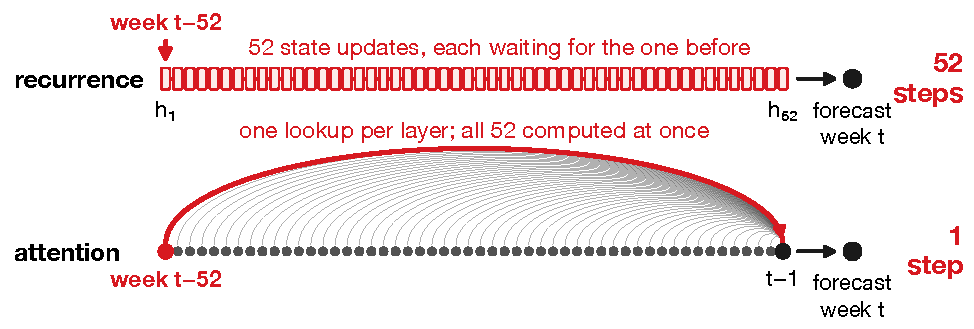
\includegraphics[height=3.8cm]{../Figures/Lecture09_Part2/recurrence_paths.pdf}
  \end{center}
  \vspace{-0.3cm}
  {\small\textbf{The information bottleneck:} week $t-52$ must survive 52 squeezes through one
  64-number state. \textbf{The sequential bottleneck:} each update waits for the last, however
  many GPUs you own.}

  \begin{keybox}
    \small\textbf{Attention removes both at once:} every week reads every other directly, and all
    are computed together. Path length counts operations, not what a trained model uses.
  \end{keybox}
\end{frame}

% =============================================================================
\section{The Attention Mechanism}
% =============================================================================

\sectionslide{The Attention Mechanism}{%
  A learned, weighted lookup --- which is a more useful way
  to read it than the formula suggests.}

% --- Slide: scaled dot-product -----------------------------------------------
\begin{frame}{Scaled Dot-Product Attention \parencite{Vaswani2017}}
  \vspace{-0.1cm}
  \[
    \text{Attention}(Q, K, V) = \text{softmax}\!\left(\frac{QK^\top}{\sqrt{d_k}}\right) V
  \]
  Each week's \textbf{query} is scored against every week's \textbf{key}, and the scores weight the
  \textbf{values}; $Q$, $K$, $V$ are learned projections of the same weeks, $d_k$ the key length.
  \begin{center}
    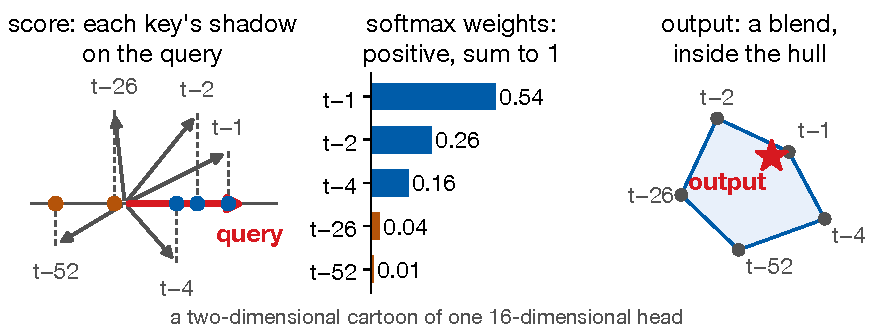
\includegraphics[height=3.4cm]{../Figures/Lecture09_Part2/attention_geometry.pdf}
  \end{center}
  \vspace{-0.3cm}
  {\small The score is the query's length times the key's shadow on it. Softmax turns the
  scores into positive weights that sum to one, so the output stays \emph{inside} the values. Attention averages; it cannot extrapolate. The $\sqrt{d_k}$ keeps the
  softmax from saturating.}
\end{frame}

% --- Slide: what it does for forecasting -------------------------------------
\begin{frame}{What That Buys a Forecaster}
  Attention can weight any week in the window in one step; an RNN needs 52 updates to reach last
  year. Where our trained model actually looked, over the test year:
  \begin{center}
    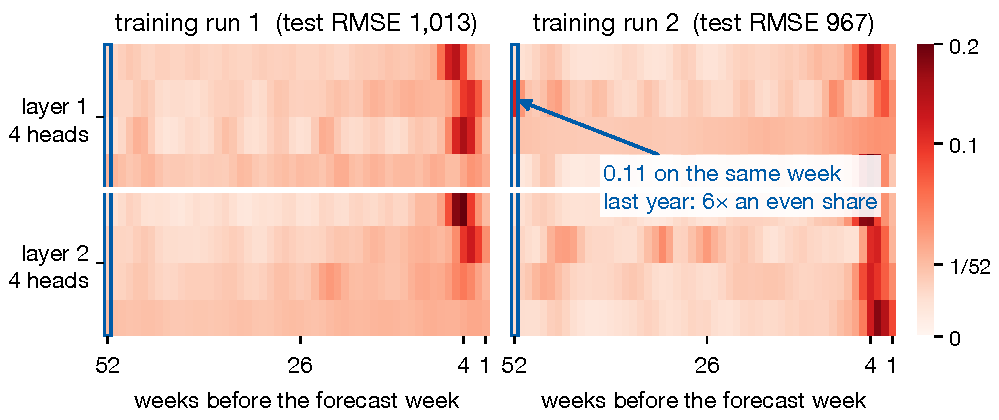
\includegraphics[height=4.2cm]{../Figures/Lecture09_Part2/attention_heatmap.pdf}
  \end{center}
  \vspace{-0.3cm}
  {\small Mostly the last two to seven weeks; in one of two training runs, one head found last
  year's week. The weights are \textbf{learned, not specified} --- and they show where the model
  looked, not what mattered.}
\end{frame}

% --- Slide: multi-head -------------------------------------------------------
\begin{frame}{Multi-Head Attention}
  One attention operation gives one set of weights --- one notion of what is relevant.
  \textbf{Multi-head attention} runs $h$ of them in parallel on different learned projections,
  then concatenates:
  \[
    \text{MultiHead}(Q,K,V) = \text{concat}(\text{head}_1, \ldots, \text{head}_h)\, W^O
  \]
  \vspace{-0.3cm}

  Each head can specialize. Ours did: most watch the last few weeks, one spreads its weight
  evenly, and in one run one found the annual lag.

  \vspace{0.15cm}
  \textbf{The cost is a surprise.} Each head works in $d_{\text{model}}/h$ dimensions, so eight
  heads cost about the same as one full-width head.

  \vspace{0.1cm}
  \muted{\footnotesize\itshape Our model: \texttt{nhead=4}, \texttt{d\_model=64} --- four heads of
  16 dimensions.}
\end{frame}

% =============================================================================
\section{The Transformer Encoder}
% =============================================================================

\sectionslide{The Transformer Encoder}{%
  Attention, plus the three pieces that make it trainable.}

% --- Slide: the block --------------------------------------------------------
\begin{frame}{The Encoder Block}
  A Transformer encoder layer is four components in a fixed arrangement:
  \begin{center}
    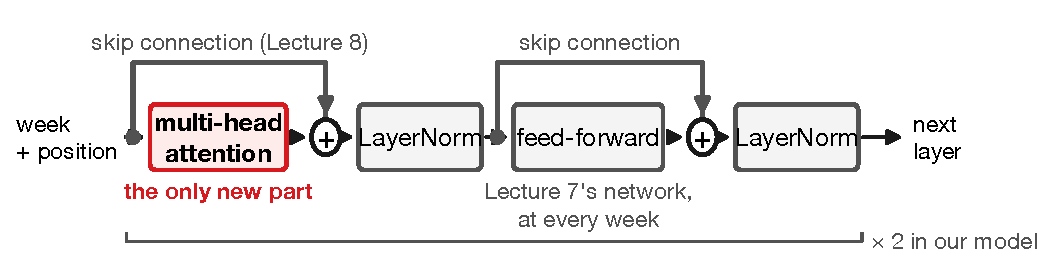
\includegraphics[height=3.4cm]{../Figures/Lecture09_Part2/encoder_block.pdf}
  \end{center}
  \vspace{-0.15cm}
  Stack $N$ of those and you have the encoder. Nothing in the block is new to you except attention
  itself --- the skip connections are ResNet's, LayerNorm rescales each week's vector, and the
  feed-forward sublayer is the Lecture 7 network applied to every week.

  \vspace{0.15cm}
  \textbf{One thing is conspicuously missing, and it is not an oversight.} Nothing above depends
  on the \emph{order} of the input.
\end{frame}

% --- Slide: positional encoding ----------------------------------------------
\begin{frame}{Positional Encoding: Attention Cannot Tell Time}
  \textbf{Attention ignores order}: shuffle the window and each week's output moves with it;
  the rest is an unordered bag. A forecaster that cannot tell two weeks ago from thirty is
  not forecasting.

  The fix adds 32 pairs $(\sin \omega_i t,\ \cos \omega_i t)$, $\omega_i = 10000^{-2i/d}$, to each
  week --- each pair a clock hand turning at its own speed:
  \begin{center}
    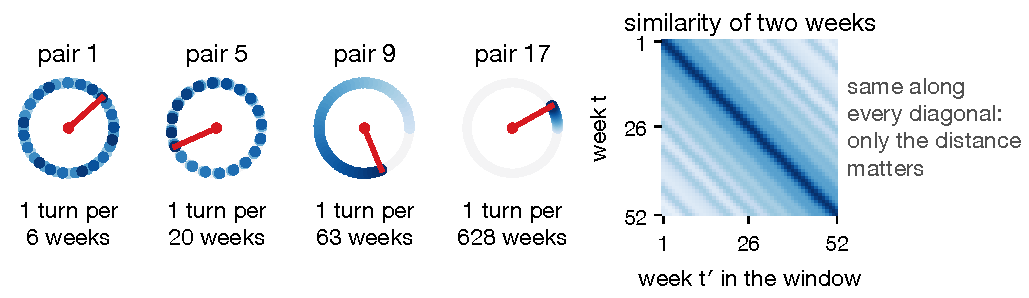
\includegraphics[height=3.5cm]{../Figures/Lecture09_Part2/positional_clocks.pdf}
  \end{center}
  \vspace{-0.3cm}
  {\small Shifting $\Delta$ weeks turns each hand by a fixed angle, so similarity depends only
  on distance. \textbf{We measure what removing it costs at the end.}}
\end{frame}

% --- Slide: why they took over ------------------------------------------------
\begin{frame}{Why Transformers Took Over}
  \begin{columns}[T]
    \begin{column}{0.47\textwidth}
      \textbf{Parallelism.} No score waits for another. More than accuracy, this is why it
      won.

      \vspace{0.15cm}
      \textbf{Direct long-range paths.} One step, any distance.

      \vspace{0.15cm}
      \textbf{Scale.} It kept improving as parameters and data grew. BERT
      \parencite{Devlin2019} and GPT are this block, repeated.
    \end{column}
    \begin{column}{0.51\textwidth}
      \centering
      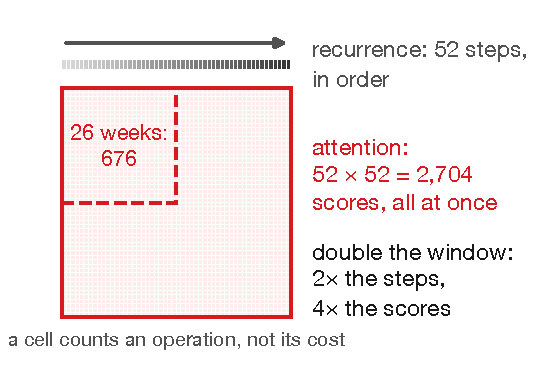
\includegraphics[height=4.4cm]{../Figures/Lecture09_Part2/attention_cost.pdf}
    \end{column}
  \end{columns}

  \vspace{0.1cm}
  {\small Each cell is one query--key score: $O(T^2)$ time and memory, fine at $T = 52$, painful
  at $T = 10{,}000$.}
  \begin{warningbox}
    \small Every advantage here is about \textbf{large data and long sequences}. Hold that
    against a 52-week window and 5{,}160 training windows.
  \end{warningbox}
\end{frame}

% =============================================================================
\section{Transformers for Time Series}
% =============================================================================

\sectionslide{Transformers for Time Series}{%
  The implementation, the measurement, and an honest reading of it.}

% --- Slide: PyTorch ----------------------------------------------------------
\begin{frame}{Transformer Encoder in PyTorch}
  \begin{examplebox}{Minimal forecasting encoder}
    {\tiny\linespread{1.15}\selectfont
    \texttt{layer = nn.TransformerEncoderLayer(d\_model=64, nhead=4,}\\
    \texttt{\mbox{}\ \ \ \ \ \ \ dim\_feedforward=128, dropout=0.1, batch\_first=True)}\\
    \texttt{self.enc = nn.TransformerEncoder(layer, num\_layers=2)}\\
    \texttt{self.inp = nn.Linear(n\_features, 64)}\\
    \texttt{self.fc\ \ = nn.Linear(64, 1)}\\[3pt]
    \texttt{def forward(self, x):}\\
    \texttt{\mbox{}\ \ h = self.inp(x) + self.pe\ \ \ \ \ \# position must be added}\\
    \texttt{\mbox{}\ \ return self.fc(self.enc(h)[:, -1, :]).squeeze(-1)}
    }
  \end{examplebox}
  \texttt{nn.TransformerEncoderLayer} gives you the whole block --- but not the positional
  encoding. You add that yourself, and forgetting is a silent failure.

  \muted{\footnotesize\itshape Multi-step forecasting also needs a causal mask.}
\end{frame}

% --- Slide: results ----------------------------------------------------------
\begin{frame}{Does It Work?}
  Same weekly panel and test block as everything since Homework 3; every sequence model reads
  52-week windows (Part 1's headline 842 and 987 were at 26 weeks).
  \begin{center}
    {\small
    \begin{tabular}{lrr}
      \toprule
      \textbf{Model} & \textbf{Test RMSE} & \textbf{Parameters} \\
      \midrule
      LASSO, 46 engineered features & \textbf{744} & 46 \\
      XGBoost & 781 & --- \\
      Vanilla RNN & \textbf{805} & 4{,}545 \\
      Random forest & 899 & --- \\
      \textbf{Transformer encoder}, 2 layers & \textbf{990} & 67{,}329 \\
      LSTM & 998 & 17{,}985 \\
      1D CNN, best variant (26-week window) & 1{,}032 & 8{,}161 \\
      Seasonal naive & 2{,}152 & 0 \\
      \bottomrule
    \end{tabular}
    }
  \end{center}

  \vspace{-0.05cm}
  The Transformer beats the CNN and \textbf{ties the LSTM} --- 990 against 998, a difference
  far smaller than the run-to-run spread. It loses to a vanilla RNN holding
  \textbf{one-fifteenth} as many parameters, and to a 46-coefficient linear model.
\end{frame}

% --- Slide: why it didn't win -------------------------------------------------
\begin{frame}{Reading That Result Honestly}
  Every advantage on the ``why Transformers took over'' slide is an advantage \emph{at scale}, and
  this problem has none of the scale.

  \vspace{0.1cm}
  \begin{center}
    {\small
    \begin{tabular}{p{4.3cm}p{8.2cm}}
      \toprule
      \textbf{Parallel computation} & Real, but irrelevant --- the RNN trains in seconds either way. \\[3pt]
      \textbf{Direct long-range paths} & Worth little when the signal is dominated by recent weeks. \\[3pt]
      \textbf{Scales with data} & 5{,}160 training windows is not the regime where that pays. \\
      \bottomrule
    \end{tabular}
    }
  \end{center}

  \vspace{-0.05cm}
  \textbf{And positional encoding is doing real work, which we can measure.} Remove it and the
  model still knows the last week, where it reads out, but sees the other 51 as an unordered
  bag:
  \begin{center}
    {\small
    \begin{tabular}{lr}
      \toprule
      Transformer \textbf{with} positional encoding & \textbf{990} \\
      Transformer \textbf{without} positional encoding & 1{,}282 \\
      \bottomrule
    \end{tabular}
    }
  \end{center}

  \vspace{-0.05cm}
  \textbf{292 RMSE} --- dropping it below even the 1D CNN. That gap is what the order of those 51
  weeks is worth, and the reason the sinusoids exist.
\end{frame}

% =============================================================================
\section{Key Takeaways}
% =============================================================================

\sectionslide{Key Takeaways}{%
  Six architectures, one series, and what the ranking actually taught us.}

% --- Slide: full comparison ---------------------------------------------------
\begin{frame}{Sequence Architecture Comparison}
  \begin{center}
    {\small
    \begin{tabular}{llll}
      \toprule
      \textbf{Architecture} & \textbf{Long range} & \textbf{Parallel} & \textbf{Needs} \\
      \midrule
      1D CNN & receptive field only & yes & modest data \\
      Vanilla RNN & $\sim$10--30 steps & no & modest data \\
      LSTM & hundreds of steps & no & more data \\
      Transformer & unlimited, $O(T^2)$ & \textbf{yes} & \textbf{much more data} \\
      \bottomrule
    \end{tabular}
    }
  \end{center}

  \vspace{0.15cm}
  \textbf{Choose by the structure of your problem, not by recency of the architecture.} Short
  window and recent-lag signal: a plain RNN, or honestly a linear model. Long sequences, abundant
  data, dependencies at arbitrary distance: a Transformer, and nothing else comes close.

  \vspace{0.15cm}
  That second case is language, which is why this architecture reshaped that field and has been
  slower to displace gradient boosting in tabular forecasting --- where the M5 competition was won
  by gradient-boosted trees, Lecture 5's method.
\end{frame}

% --- Slide: takeaways --------------------------------------------------------
\begin{frame}{Lecture 9, Part 2: Key Takeaways}
  \begin{keybox}
    {\small
    \begin{enumerate}\itemsep3pt
      \item \textbf{Attention}: score queries against keys, softmax, average the values.
      \item Its price is \textbf{quadratic}: fine at 52 steps, the central constraint at
            10{,}000.
      \item \textbf{Multi-head}: several notions of relevance for about the cost of one.
      \item An encoder block: attention, \textbf{skips}, LayerNorm, feed-forward. Only
            attention is new.
      \item \textbf{Attention ignores order}: add position yourself; PyTorch will not.
      \item Here it \textbf{tied the LSTM} and lost to an RNN \textbf{one-fifteenth} its size:
            it needs scale.
    \end{enumerate}
    }
  \end{keybox}
  \muted{\itshape Next: Bayesian Statistics I --- a different answer to what a forecast should
  tell you.}
\end{frame}

% --- References ---------------------------------------------------------------
\begin{frame}[allowframebreaks]{References}
  \printbibliography[heading=none]
\end{frame}

\end{document}
